% Created 2022-10-16 Sun 21:58
% Intended LaTeX compiler: pdflatex
\documentclass[11pt]{article}
\usepackage[utf8]{inputenc}
\usepackage{wrapfig}
\usepackage{indentfirst}
\usepackage{rotating}
\usepackage[normalem]{ulem}
\usepackage{amsmath}
\usepackage{amssymb}
\usepackage{amsfonts}
\usepackage{hyperref}
\usepackage{tikz}
\usetikzlibrary{shapes,arrows,positioning,calc,chains,decorations.pathreplacing}
\usepackage{listings}
\usepackage{color}
\usepackage[utf8]{inputenc}
\usepackage[margin=1.0in]{geometry}
\usepackage{subcaption}
\usepackage{}

\captionsetup{width=.75\textwidth,font={small},labelfont=bf}

\hypersetup{
 pdfauthor={Ben Anderson},
 pdftitle={UR3e Documentation},
 pdfkeywords={},
 pdfsubject={},
 pdflang={English}}
\begin{document}

\tikzset{
block/.style = {draw, fill=white, rectangle, minimum height=3em, minimum width=3em},
tmp/.style  = {coordinate}, 
sum/.style= {draw, fill=white, circle, node distance=1cm},
input/.style = {coordinate},
output/.style= {coordinate},
pinstyle/.style = {pin edge={to-,thin,black}
}
}
\newcommand\connect[2]{\path[draw,arrow] (#1) |- ($(#1)!1/2!(#2)$) -| (#2)}
\newcommand\ImageNode[3][]{
  \node[draw=arrowblue!80!black,line width=1pt,#1] (#2) {\includegraphics[width=1.5cm,height=1.5cm]{#3}};
}

\date{\today}
\author{Ben Anderson}
\title{The STANLEy User Manual \\[1ex] \large Stabilization and Transducer Alignment for Nearby Laser Elastography}
\maketitle
\tableofcontents
\parskip=6pt

\section{Introduction}\label{sec:intro}

The focus of my work for the better part of the last year has been studying how to use a UR3e Cobot for the purposes of focusing and stabilizing a sensor at its focal length away from a target surface. This has involved a thorough examination of the API and programming tools that accompany the Universal Robots ecosystem, as well as creating systems for synchronizing the robotic control system with signal processing and sensor systems.

In doing so a number of systems are being used in ways for which they were not designed. The consequence of this is that my codebase resembles a kludgy pile of half-fixes and temporary-solutions that, technically, have achieved the objective, at the expense of stability and ease of use.
In recent months more efforts have been made to improve the readability of the codebase and allow for easier changes later on, but the work is ongoing and the project cannot wait for me to complete this work.

The hope is with this documentation, others in the OCE project can gain enough of an understanding of how the system works to use it in my absence as well as modify or extend the platform I've built.

Due to the kludgy nature of the platform, it may not be suitable to read this guide linearly. The introduction section should hopefully give you an overview of how the components of this section communicate and interface with each other, and a more thorough description of the workings of each module are in the following chapters.

If your only goal is to get started running the robot, strictly speaking you need only read the startup section (\autoref{sec:startup}), though I recommend also reading \autoref{sec:pendant}, which covers use of the teach pendant.

If you need to 

\section{Startup guide}\label{sec:startup}
Pending the rest of the summary, the following procedure should be all you need to start running this control system on your machine.
\subsection{First installation}
These steps only need to be ran once when initially setting up your Cobot, and don't need to be repeated on subsequent use.
\begin{enumerate}
    \item Install all software dependencies on the computer.
    \begin{itemize}
        \item Python 3.8+ on target machine
        \item Packages required for all of the python code can be installed by running \\ \texttt{pip install -r requirements.txt} \\ from the main directory of this repository
        \item MATLAB/LabView/whatever other signal processing code you need for dealing with sensor input
    \end{itemize}
    \item Connect the UR3e robot to your machine via an ethernet cable.
    \item Assign the ethernet connection to your robot a static IP address with the following criteria:
    \begin{itemize}
        \item \textbf{IPv4}
        \item \textbf{IP address:} \texttt{192.168.0.5} (Corresponds to addresses hard-coded into the running programs)
        \item \textbf{Subnet prefix length:} \texttt{255.255.255.0}
        \item \textbf{Gateway:} \texttt{192.168.0.1}
        \item \textbf{Preferred DNS:}  \texttt{10.1.2.1}
        \item \textbf{Alternate DNS:} \texttt{8.8.8.8} (Less critical, any valid DNS will do)
    \end{itemize}
    \item Do the same on the robot, instead assigning the following values:
    \begin{itemize}
        \item \textbf{IPv4}
        \item \textbf{IP address:} \texttt{192.168.0.10}
        \item \textbf{Subnet prefix length:} \texttt{255.255.255.0}
        \item \textbf{Gateway:} \texttt{192.168.0.1}
        \item Set the DNS settings to any valid DNS addresses.
        \item Details on modifying network settings an be found on page 108 of the \hyperlink{https://s3-eu-west-1.amazonaws.com/ur-support-site/44018/Software_Manual_en_Global.pdf\#page=108}{Polyscope manual}
    \end{itemize}
    \item Write/save/open a program on the UR3e that does the following:
        \begin{quote}
\begin{verbatim}
BeforeStart:
    script(before_start.script)
Robot Program:
    script(robot_program.script)        
\end{verbatim}
        \end{quote}
    \begin{itemize}
        \item The corresponding scripts are found in the \texttt{\textbackslash{}Code\_for\_the\_robot} folder in this repository.
        \item For more information on node programming, check out the chapter on programming in the \hyperlink{https://s3-eu-west-1.amazonaws.com/ur-support-site/44018/Software_Manual_en_Global.pdf\#page=60}{Poylscope manual} 
    \end{itemize}
    \item Make sure the robot has the correct installation selected. This includes making sure the dimensions of the tool match the current setup of the sensor on the end effector of the robot. For more information on configuring the tool, read the section on TCP configuration in the \hyperlink{https://s3-eu-west-1.amazonaws.com/ur-support-site/44018/Software_Manual_en_Global.pdf\#page=73}{Polyscole manual}
    \begin{itemize}
        \item This will require some knowledge of the shape/orientation of the sensor you are currently working with.
        \item When working with sensors that have a focal point offset from the end of the tool, the TCP offset should be defined at the location of the focal point, not the edge of the tool.
    \end{itemize}
\end{enumerate}
This setup will only need to be run when a part of your installation changes. Steps one through three need to be repeated whenever you run the installation on a new computer; step four only needs to be run once for each robot (or whenever the robot goes through a hard-reset).
Steps five and six shouldn't \textit{need} to be repeated regularly, but sometimes need to be rerun if the robot isn't shut down correctly. (This is very easy to do).
\subsection{Starting up the robot}
Once the above configuration steps have be completed, you should be ready to run experiments with the robot after following this procedure:
\begin{enumerate}
    \item Power on the robot by following the boot-up procedure described in \autoref{sec:powerup} (also power on your computer, obviously)
    \begin{quotation}
        \textbf{Warning}: The robot will move slightly when it boots up as it unlocks its brakes. Keep sensitive equipment clear from the robot, and do not power off the robot in a position that will put nearby objects at risk when it is turned on.
    \end{quotation}
    \item (Optional) Use the teach pendant to manuever the robot into a position convenient for the following test. This is optional as the control loop allows you to toggle freedirve mode, but it may be more convenient to do so here.
    \item Make sure the correcet program and installation are selected on the teach pendant; To read more about navigating the program/installation menus, read the section on this subject in the \hyperlink{https://s3-eu-west-1.amazonaws.com/ur-support-site/44018/Software_Manual_en_Global.pdf\#page=103}{Polyscope Manual}
    \item Do any setup necessary for your sensor now; the robot can be left idle while you do so.
    \item Once your setup is ready, open the \texttt{COBOT\_Transducer\_Control\_Code} directory on your PC, and double-click \texttt{server.py}
    \begin{itemize}
        \item A blank terminal window should pop up with a blinking cursor; (You do not need to interact with the terminal window, it is only there for status messages)
        \item This activates the socket server that the system uses to communicate between modules.
    \end{itemize}
    \item Tap the `play' button at the bottom of the teach pendant to run the program; The terminal window from the previous step shold show a new connection has been established.
    \item Start your signal processing script; make sure your signal processing program follows the appropriate data transmission standard (Described in \autoref{sec:data_format_fig}) (TODO elaborate)
    \item Finally, run \texttt{TransducerHoming.py}. This can be done by double-clicking the file in file explorer, but it is better to run it from an IDE such as Visual Studio; the software is not stable and being able to see an error message when it breaks is very helpful.
    \begin{itemize}
        \item This should open a terminal window that looks like the following:
    \end{itemize}
\begin{verbatim}
TCP position in relation to its initial position:
        ([[-1000.00 -1000.00 -1000.00]](mm),[[-57.30 -57.30 -57.30]](deg))
=========================
TCP position in base: ([[ 0.00  0.00  0.00]], [[ 0.00  0.00  0.00]]
Current joint position in degrees: ([[ 0.00  0.00  0.00  0.00  0.00  0.00]])
Recent refresh rate: 0.1465371191501617415
------------------------
Latest mag:48
|||||                                                                      |
Freedrive active: False
Press (f) to toggle (f)reedrive mode :)

Press (d)emo to demonstrate the basic pathrouting module
Press (k) to trigger a full scan with hard-coded resolution.
Press (g) to trigger a amplitude max-finding pathrouter.
Press (t) to trigger an alternate amplitude max-finding pathrouter.
Press (q) to quit

Sun Nov 20 18:23:36 2022
----------------
\end{verbatim}
\end{enumerate}

From here you are ready to run your test. Follow the directions on screen to enable/disable freedrive and activate the appropriate pathfinding module. The two menu options I suggest using are `(k) for fullscan' and `(g) for maxfinding'. The fullscan module runs a full scan of a search volume of a hard-coded shape and resolution, and the maxfinding module runs the current-best module for focusing a transducer.
\subsection{Common debugging steps}
Because the sole author of 90\% of this code is such a genius, occasionally this software breaks in ways that may be frustrating. Here are common problems and the best-known steps to address them (short of writing better sofware)
\begin{itemize}
    \item The robot collides with something during a test and locks itself up
    \begin{enumerate}
        \item If this happens the experiment is ruined, you will need to restart
        \item Close the \texttt{TransducerHoming.py} script, and stop the socket server.
        \item The robot will need to be unlocked through the main menu, after you have done so tap the `stop' button to cancel the running program (the default behavior is to pause the program, you don't want that)
    \end{enumerate}
    \item \texttt{TransducerHoming.py} crashes
    \begin{itemize}
        \item This is a frequent occurance whenever major changes are made to the program or installation
        \item It is worth noting though, that \texttt{TransducerHoming.py} is not a dependency for the other components; they will simply sto pmoving. You are able to restart the script without resetting any of the other systems.
        \item If you ran the script through an IDE, take note of the error message and where it occured, and alert Ben Anderson to the problem (bpa13@uw.edu) or submit a pull request on github
    \end{itemize}
\end{itemize}

\section{System Overview}
\begin{figure}[ht]
\centering
\begin{tikzpicture}[auto, node distance=3cm, on grid,auto,>=latex']
\node[block] (sensor) {Sensor};
\node[block, right = of sensor] (robot) {UR3e};
\node[block, right = of robot] (URScript) {URScript};
\node[block, below = of sensor, align=center] (labview) {Signal\\Processing};
\node[block, right = of labview, align=center] (socket) {Socket\\Server};
\node[block, right = of socket, align=center] (tcc) {Control\\Code};

\draw [draw, <-] (robot) -- (URScript);
\draw [->] (sensor) -- (robot);
\draw [draw, <->] (sensor) -- (labview);
\draw [->] (labview) -- (socket);
\draw [<->] (socket) -- (tcc);
\draw [<->] (socket) |- ($(socket)!1/2!(socket |- URScript)$) coordinate (C) -| (URScript);

\node[text=black, below left= 6mm and 12mm of tcc.west] (pc) {PC};
\draw[black, dashed] (pc.east)-|([xshift=3mm]tcc.east)|-([yshift=3mm]socket.north)-|([xshift=-4mm]labview.west)|-(pc.west);

\node[text=black, above right= 6mm and 4mm of robot.east] (ur) {STANLEy};
\draw[black, dashed] (ur.east)-|([xshift=3mm]URScript.east)|-([yshift=-3mm]robot.south)-|([xshift=-4mm]robot.west)|-(ur.west);

\end{tikzpicture}
\caption{Component overview of the STANLEy system}\label{fig:component_block_diagram}
\end{figure}
The system is designed to keep as much modularity as possible and to isolate responsibilities for particular tasks.

The sensor is a generic device that requires focusing and produces an output that is read by the signal processing package within the computer. The Stabilization and Transducer Alignment for Nearby Laser Elastography system (hencforth referred to as STANLEy) consists of a UR3e cobot from Unviersal Robots, and a script written in using the Universal Robots proprietary scripting language.
(Attempts are being made to reverse-engineer some of this languages functions to cut this box out of the control diagram, but the process will be very involved and is being put off in order to meet deadlines).

Physically, this system includes a robotic arm manipulator, a control box, and a teaching pendant.
STANLEy interfaces with the sensor through a physical linkage at the end of the robotic manipulator, and with the PC through an ethernet cable.

The remaining control blocks occur within a nearby computer. The signal processing block refers to a program (typically in MATLAB or LabView) which recieves the data from the sensor and processes it for further use. 

\textbf{For the purposes of the control loop that focuses the sensor, the signal processing block must reduce the sensor input, no matter how complex, to a simple magnitude that should be maximized to bring the sensor into alignment.} More on this to be added later.

An internal socket server is spun up in a simple python program.
This is a program that listens on a hard-coded IP-address and port within the computer for input sent from the signal processing block, the control code, and to the robot through the control box.
More on the specific IP addresses in the initial setup section of the startup section. (\autoref{sec:startup})

The control code is run from a script named \texttt{TransducerHoming.py}, and associated libraries. For now, directly editing this file is the main interface with which we can modify how the homing sequence runs.
In future I hope to expand the user interface as well as the command-line options to allow more on-the-fly modification of program parameters, but the duration off tests and the speed at which changes are made have made this an inefficient goal for some time.

Overall the system utilizes three discrete devices and at least three programming languages. I (Ben Anderson) am most directly involved with the programming of the control code and URScript. The top-down overview of each components' functions are pretty simple, but debugging/modifying them will require a rough understanding of the URScript API and a strong understanding of Python.

\section{STANLEy and the URScript API}\label{sec:robot_summary}
The body of the novelty surrounding this project centers around the use of a UR3e robotic arm to position and hold the OCE sensor.

The UR3e is manufactured by Universal Robots and is primarily designed to automate human labor. Shipped with the robotic arm is a control box and a teach pendant, a hand-held tablet for manually controlling the robot. The control box allows one to write and execute scripts using the proprietary URScript API, a set of functions built into the robot that handle common tasks related to positioning and animating the arm.

Additionally, the control box has an ethernet port supporting the secondary and Real Time Data Exchange interfaces. Both of these have their uses and can be read about in the \hyperlink{https://www.universal-robots.com/articles/ur/interface-communication/remote-control-via-tcpip/}{remote control interface guide}, however they weren't adequate for the method ultimately used.

\subsection{The Teach Pendant and the PolyScope interface}\label{sec:pendant}
The teach pendant is the default accesory for interacting with the internals of the robot. It is shipped with the robot along with the control box.
\begin{center}
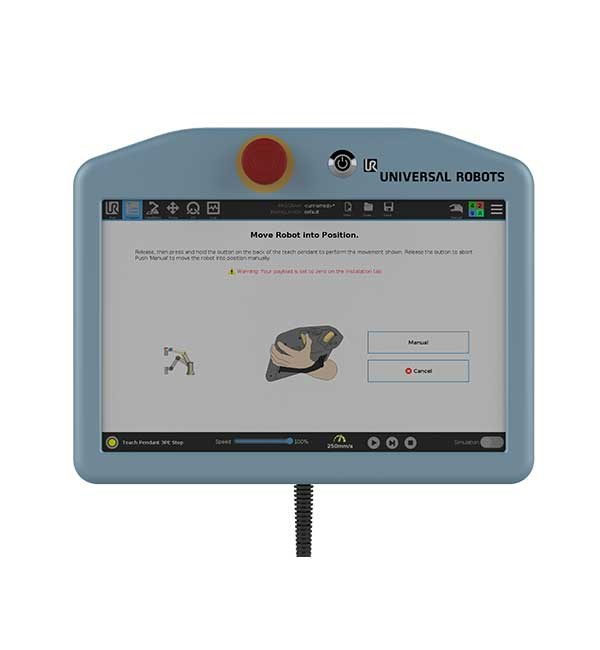
\includegraphics[width=.5\linewidth]{figures/teach_pendant.jpg}
\end{center}
The pendant, when active, is running an interface known as PolyScope, the GUI used for operation of all UR robots. Along the top of the page, there are six different menus and a file explorer interface that we will refer to later:

\begin{center}
\includegraphics*[width=\linewidth]{figures/menu_banner.jpg}
\end{center}

The full manual for PolyScope can be read \hyperlink{https://s3-eu-west-1.amazonaws.com/ur-support-site/114079/99403_UR3e_User_Manual_en_Global.pdf\#page=107\&zoom=100,76,233}{here}, but this guide will cover the elements necessary for operation of STANLEy.

\subsubsection{Initialization and setup}\label{sec:powerup}
In order to use the robot, power on the tool box by pressing the physical power button above the screen and next to the e-stop on the teach pendant. 
(It can be finicky how long a press is necessary, so if you suspect you're holding the button down too long listen for a click from the control box to indicate it has been powered on. You should release the button immediately after hearing this click).

The power button should light up green and the screen should show a loading screen as the robot takes a minute to boot up.

Upon fully booting up, the robot itself still remains dormant. In the bottom-left of the screen is the \uline{robot status indicator}, shown here:

\begin{center}
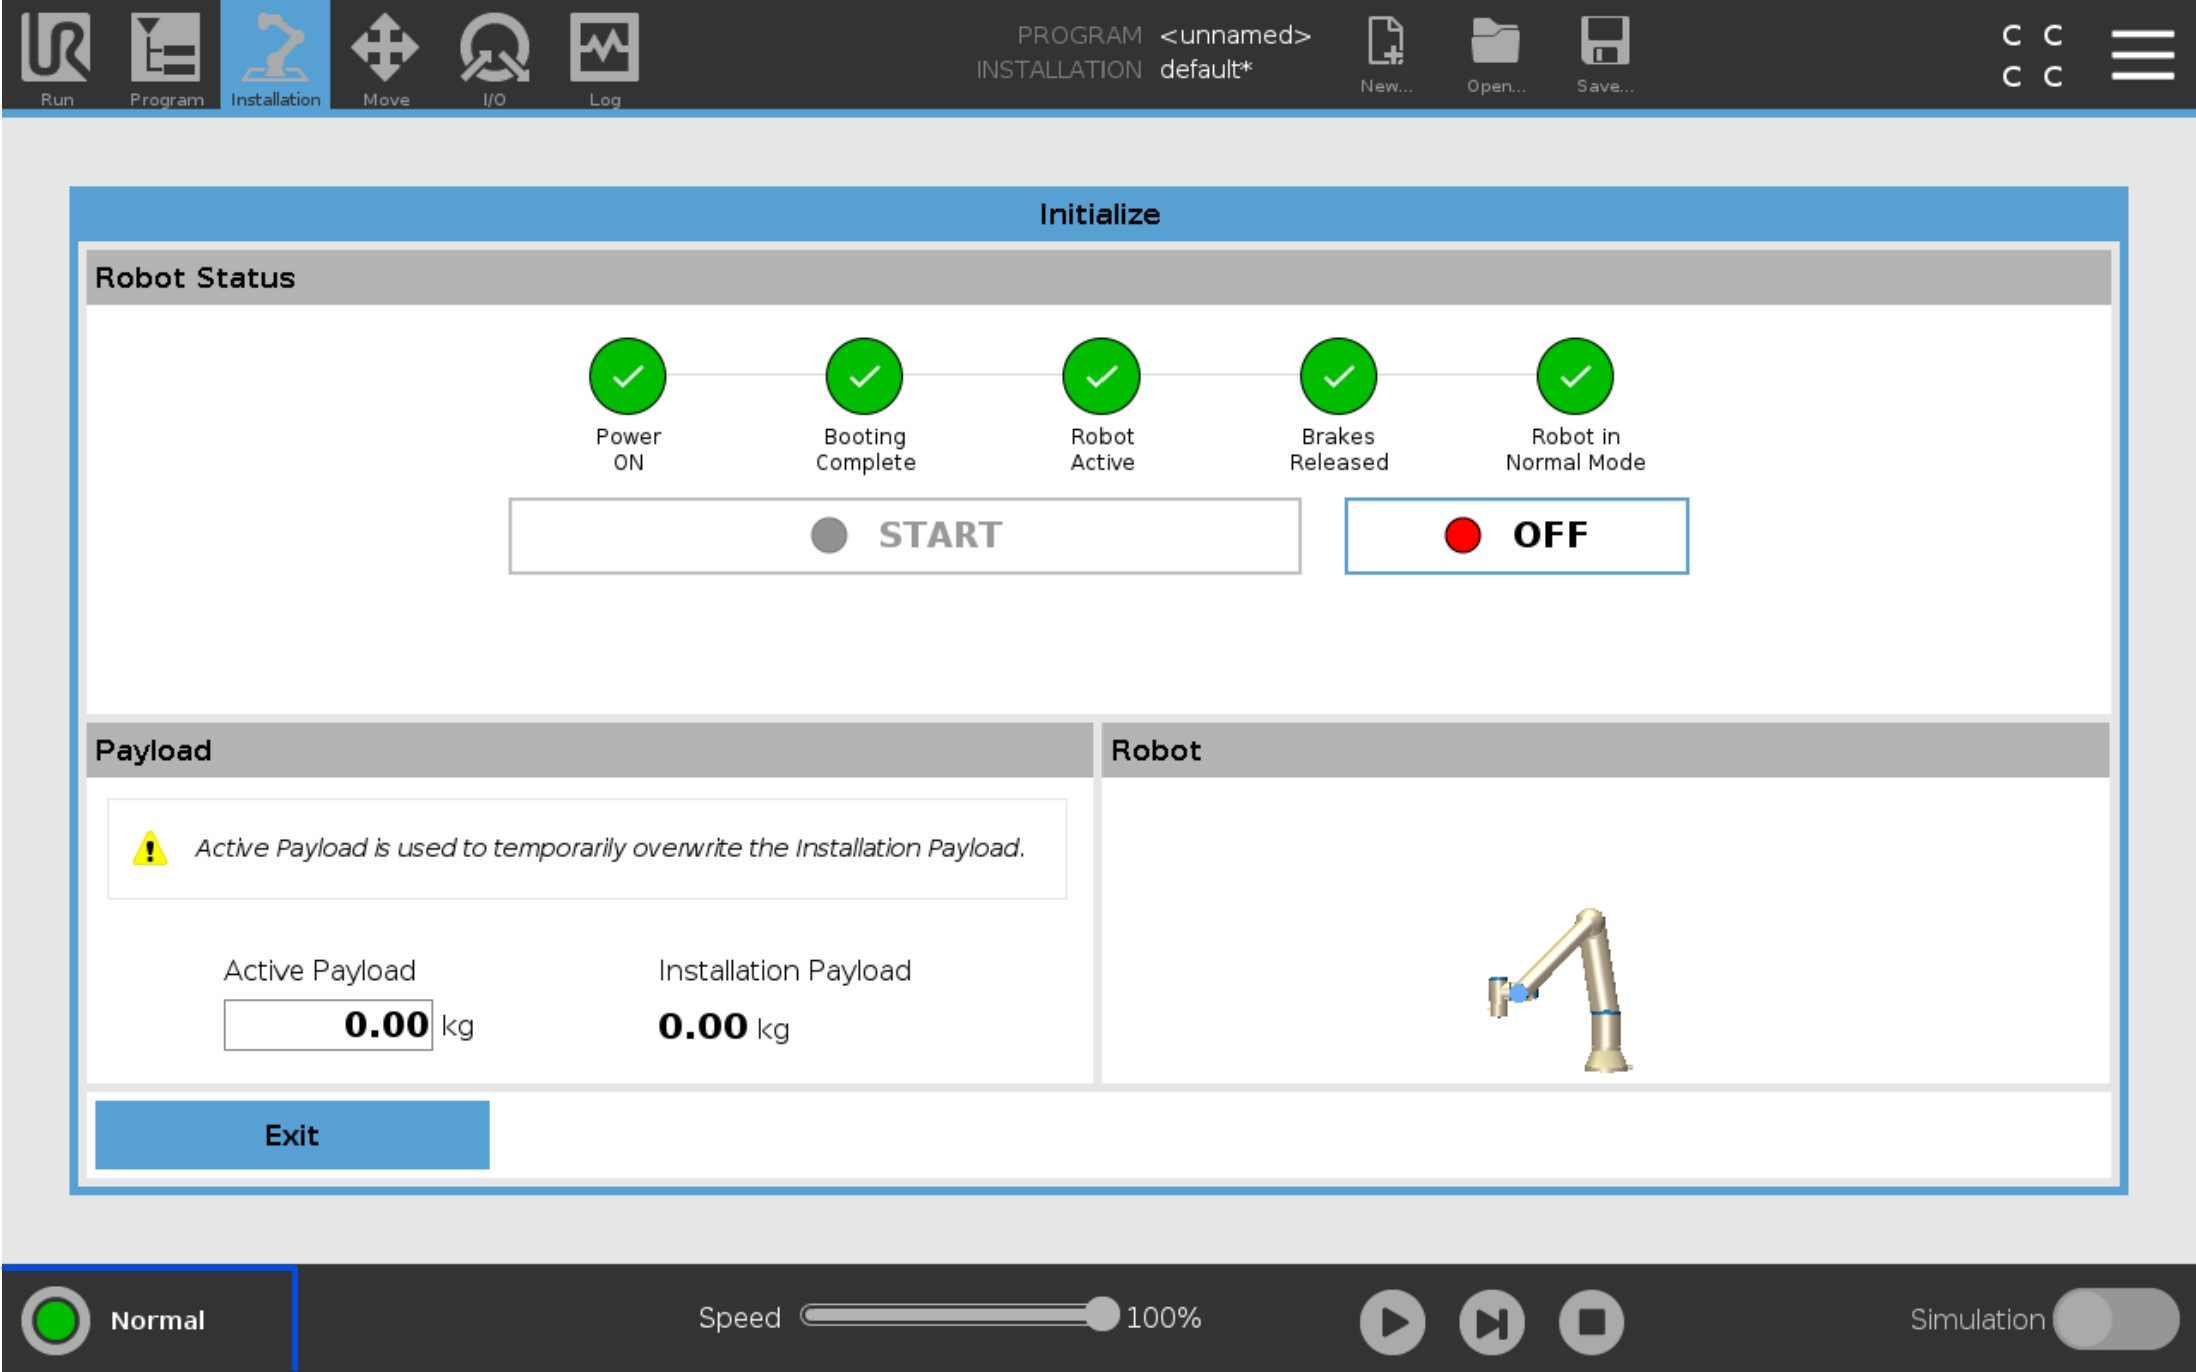
\includegraphics[width=.9\linewidth]{figures/robot_state_menu.jpg}
\end{center}

The color inside the circle indicates the state of the robot:
\begin{itemize}
    \item \emph{Red}: The robot is powered off.
    \item \emph{Blue}: The robot is in freedrive mode.
    \item \emph{Yellow}: The robot is idle; powered on but not ready for operation.
    \item \emph{Green}: Powered on and ready for normal operation.
\end{itemize}

After booting up the control box you enter the Initialization screen (shown in the image above). When powering up the robot from full-shutdown the central button will be active and you will press it twice to enable the robot; first it will say `ON' and you press it to deliver power to the robot, then it will say `START' and you will press it to unlock the brakes and enable the robot completely.

\textit{\textbf{Warning:}} The robot will move slightly as the brakes are unlocked, do not leave the robot in a stat where this motion will put nearby equipment at risk.

\subsubsection{Program tab}
The \hyperlink{https://s3-eu-west-1.amazonaws.com/ur-support-site/44018/Software_Manual_en_Global.pdf\#page=103}{program tab} is one of the options in the menu tab. Here is where you write/modify programs for controling the robot.
Polyscope has a node-based programming langauge similar to scratch, in addition to a powerful scripting language that can be baked into a robot program.
When you press the `play' button at the bottom of the tablet, the program it runs will be in this form (if one is loaded).

Stanely (The UR3e currently used in our lab) has a program saved called \texttt{test.urp} that works with our control code.
It can be opened by tapping the `open' button in the top banner and tapping `Program' from the subsequent dropdown. 
Our program relies heavily on the scripting language, so the only nodes in our program are a `BeforeStart' and `Run Program' node, each containing a script that does everything we need.
\begin{quote}
\textbf{Note}: If you want to edit either of these programs, \textit{use a USB stick and a computer to transfer/edit the program}. The text input for the teach pendant is a finicky touch screen and I've had trouble getting a keyboard with the right language settings.
\end{quote}

\subsection{URScript API}\label{sec:urscript}
URScript is the propreitary scripting language created by Universal Robots and runs natively on all of their machines. The functions are tailored to work for their machines specifically, and I haven't found a way to run URScript outside of the control box.
The full URScript API guide can be found \href{https://s3-eu-west-1.amazonaws.com/ur-support-site/32554/scriptManual-3.5.4.pdf}{here} (a copy of this document can also be found in Documentation folder of this git directory).

The URScript API provides one major opportunity and one major problem; On the one hand, it abstracts-away a lot of the low-level handling that's required to move the robot in a controlled manner. At no point in this project did we need to work with inverse kinematics or joint positions or anything of that sort.

The tradeoff is that the URScript API is extremely confining and doesn't provide a lot of ways to interface with other computers. The UR series of robots were designed to work collaboratively with humans, automating tasks that would normally be done with manual labor. Consequently, most of the scripting language and interfaces are designed with repetitive, simple tasks in mind, and getting the robot to work in an active control setting was a challenge.

Essentially the two ways they design the robot to work is either as a standalone machine, running URScript program nodes that get written once and then repeated forever, or as a mindless drone recieving simple commands from an external computer.

There is an interface in the robot to allow for direct control from an external computer, but the available commands in this mode are limiting.
\section{Control code}\label{sec:control_code}
Working on it
\begin{center}
    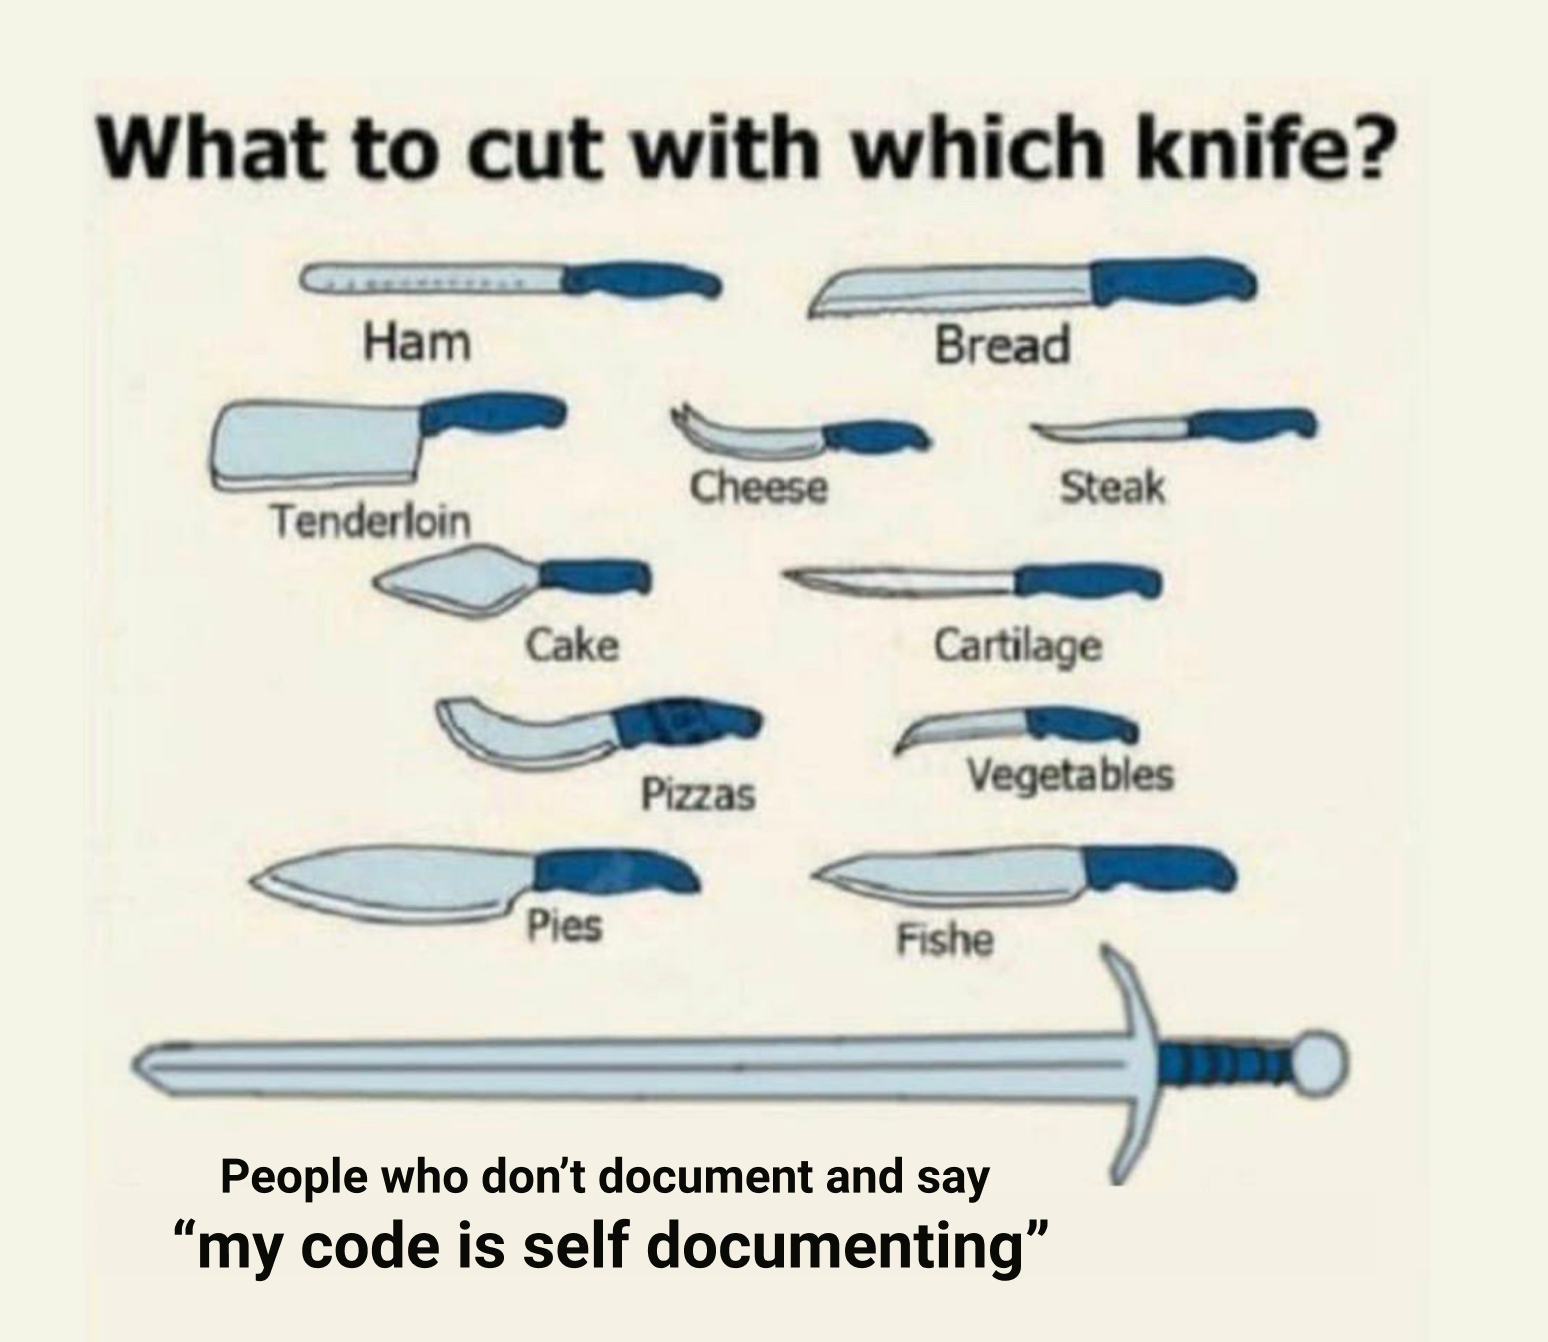
\includegraphics[width=.6\linewidth]{figures/control_code_loading_image.png}
\end{center}

\subsection{\texttt{TransducerHoming.py}}\label{sec:TransducerHoming}
476 lines of nonsense and yes I wrote the whole thing myself. No I am not fine. More extensive documentation is pending but for now we need only refer to the data formatting standard used to pass data between the sensor and the control code: \autoref{sec:data_format}

STANLEy -\> Stabilization and Transducer Alignment for Nearby Laser Elastography

\subsubsection{Interfacing with Sensor output}\label{sec:data_format}
The control code has been written to move the robot in such a way that it maximizes some value it is getting passed from the outside. It is completely agnostic about where this value comes from, and it is the programmers responsibility to ensure that the value it gets passed is an appropriate function of how `focused' the sensor you're working with is.

Our goal is to create a fitness function $f$ that produces a single scalar value representing how well focused the sensor is. A fitness function $f$ will result in the robot focusing correctly if:
\begin{itemize}
    \item The global maximum value of $f$ occurs at the focal point of the sensor
    \item $f$ has few or no local maxima
\end{itemize}
Other desireable properties of the fitness function are:
\begin{itemize}
    \item Function $f$ is concave (e.g. $\nabla^2 f \leq 0$ for everywhere in the domain)
    \item $f$ has a discrenable magnitude for a wide envelope around the focal point (since eventually the function will be dominated by noise)
    \item $f$ has a high SNR across as much area as possible
    \item $f$ is smooth everywhere
    \begin{itemize}
        \item If $f$ is smooth everywhere except at the focal point $f_{\max}$, that is also acceptable
    \end{itemize}
\end{itemize}
The robot control code sees this value as some function of the tools position in 6-D space, and will try to maximize that function according to the constraints you give it.

Once that fitness function has been defined, the signal-processing toolkit must send that value to the central socket server as a string in the following format:

\begin{figure}[ht]
    \begin{center}
        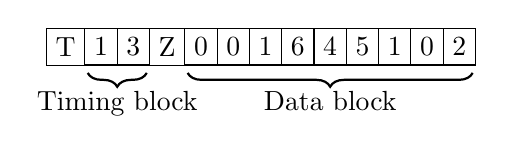
\begin{tikzpicture}[
            node distance=0pt,
            start chain = A going right,
                X/.style = {rectangle, draw,% styles of nodes in string (chain)
                            minimum width=2ex, minimum height=3ex,
                            outer sep=0pt, on chain},
                B/.style = {decorate,
                            decoration={brace, amplitude=5pt,
                            pre=moveto,pre length=1pt,post=moveto,post length=1pt,
                            raise=1mm,
                                        #1}, % for mirroring of brace, if necessary
                            thick},
                B/.default=mirror, % by default braces are mirrored
                ]
            \foreach \i in {T,1,3,Z,0,0,1,6,4,
                            5,1,0,2}% <-- content of nodes
                \node[X] {\i};
            \draw[B] (A-2.south west) -- node[below=2mm] {Timing block} ( A-3.south east);
            \draw[B] (A-5.south west) -- node[below=2mm] {Data block} (A-13.south east);
        \end{tikzpicture}
        \caption{Visual description of the data format in messages between the sensor processing block and the socket server.}\label{sec:data_format_fig}
    \end{center}
\end{figure}
The two characters following the $T$ is a timing block that increments by one each time a new value is sent to the server (this is so the code knows when a value it recieves is new). The nine characters following the $Z$ is the data block, and this is where the value of the fitness function must go. Nine digits is an arbitrary choice of precision, but should be sufficient for the kind of resolution we deal with.
\begin{quote}
    \textbf{Note:} The socket server can only handle integers, but high-resolution data can still be provided by multiplying a value by some large number before passing a value in.
\end{quote}
For example, my previous setup yielded fitness values in a range between $40$ and $700$, so to capture full definition I multiplied the value by $1000$ before passing it and divided it again on the other side.


\section{Testing methodology}
The control logic we write for focusing the transducer needs to be resilient to noise and different initial placements of the sensor. Therefore it is critical that each mode of control logic gets tested thoroughly before being relied on in produciton.
There are logistical limitations with testing control logic exclusively on the physical system, and if a particular algorithm fails to focus the transducer correctly, it's not always possible to understand why.

To deal with this, control patterns were tested against pre-recorded data so their feasability could be checked quickly, before the simulated results were validated with the real robot.

The \texttt{FullScan} module in \texttt{Pathfinders.py} defines a pathfinder that visits every point in an n-dimensional search space at a given resolution. Such resolution should be adjsted to reflect the size of the focal area of the sensor.

Shown below is the data in \texttt{test\_6.json}, which captured over $51749$ signal magnitudes. It scanned a search space that spanned $\pm 13^\circ$ in the $\theta_x,\theta_y$ directions, and $\pm 14 mm$ in the $z$ direction, at a resolution of $0.4 mm$ along translational axes and $1.0^\circ$ in the rotational axes.

\begin{figure}[ht]
    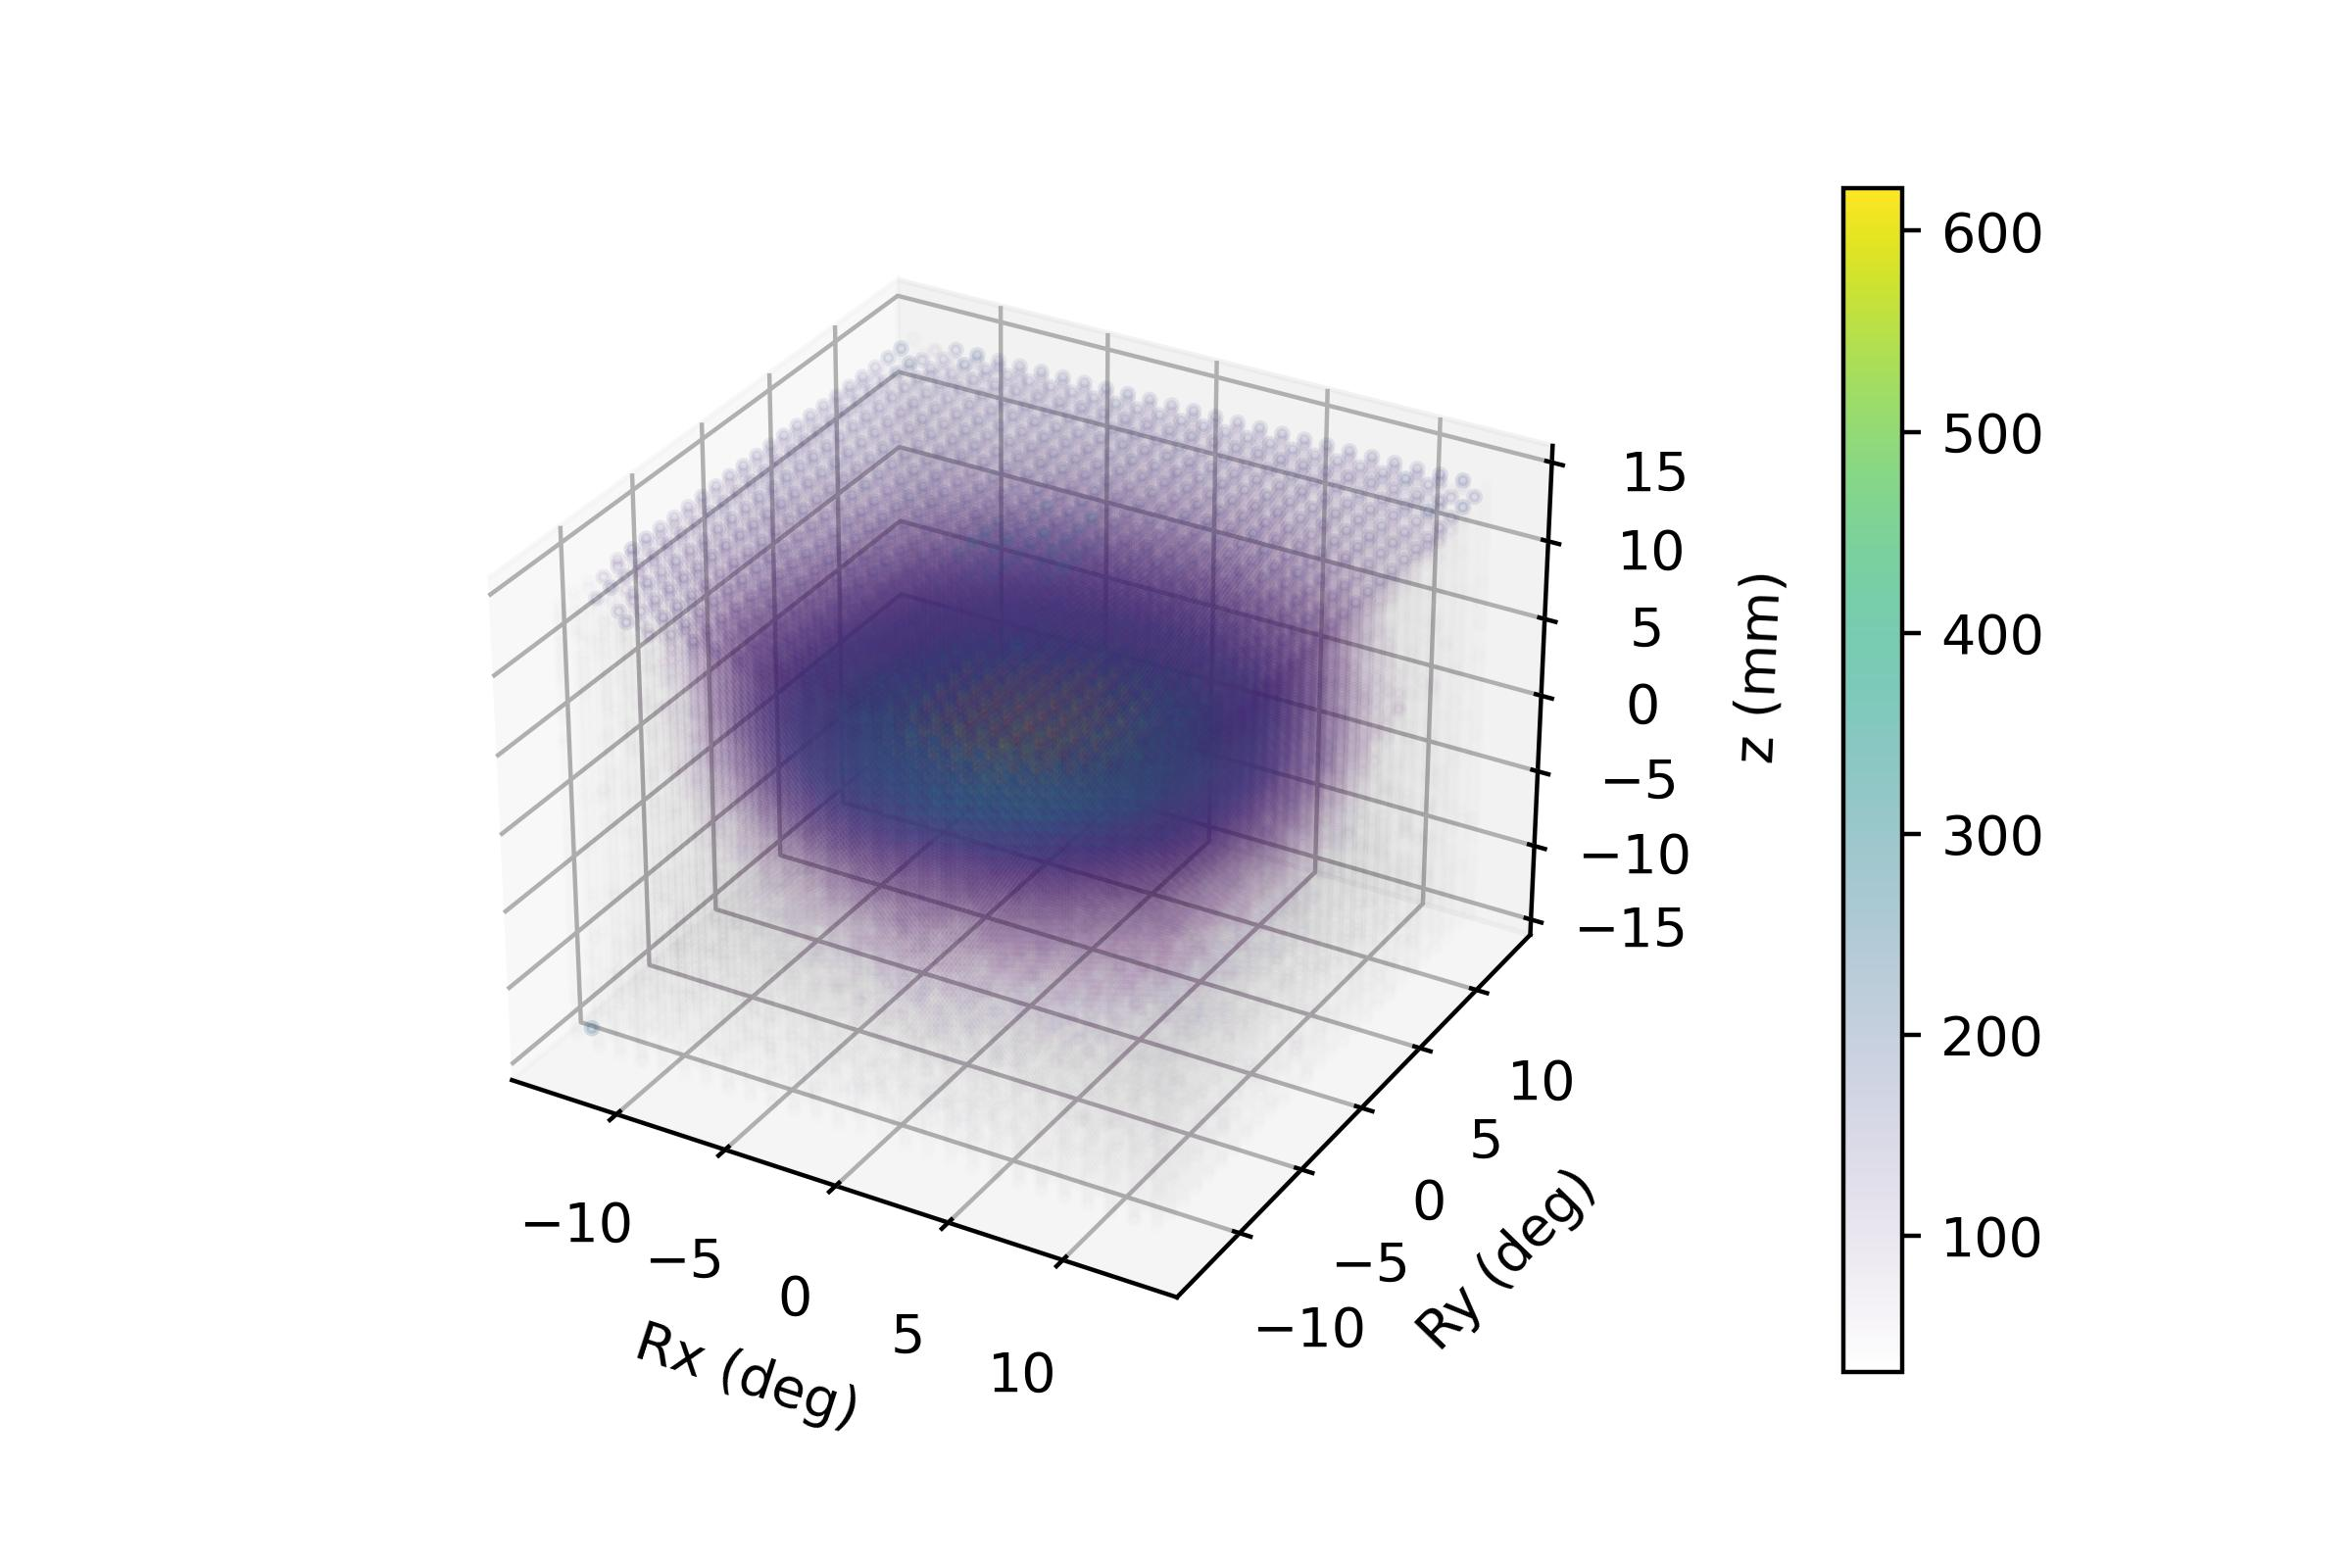
\includegraphics[width=.9\linewidth]{figures/fullscan_render_test_6.jpg}
    \caption{Raw data output from a full-scan (opacity is scaled with data magnitude, so many values are hidden)}\label{fig:fullscan-6}
\end{figure}

There are two helpful things that the data from a full scan gets used for; first of all it allows us to test our pathfinders explicitly on pre-existing data, and secondly it allows us to evaluate how our fitness function plays out in a real scan.

\subsection{Sensor fitness function}
\subsubsection{A foreword in fitness function design}
Earlier the fitness function was described as a function of the position of the robot that outputs a scalar representing how well the sensor is focused, and that the robot control code sees this as a function in 6-D space. Now we will get into the process of designing and evalutating effective fitness functions.

Since we are trying to bring a sensor into focus, we assume that the `focusedness' of the transducer is some function of its position in 6-D space relative to the target. Since, fundamentally, the focusedness of a sensor relates to some physical phenomena, we can imagine a function $\delta(\mathbf{X})$ that represents the true function mapping sensor-target position $\mathbf{X} = \{x,y,z,\theta_x,\theta_y, \theta_z\}$ to sensor focus.
This function should relate to the fundamental principles of the sensing method and the quantity being measured.

In the real world our sensor will never be able to take perfect readings because we cannot isolate the quantity being measured from the other elements of the system. Therefore we must imagine that the data collected from our sensor is some mixture of the ground truth function and some stochastic noise.

\begin{equation*}
    \mathcal{D} = \delta(\mathbf{X}) + \epsilon \qquad \epsilon \sim \mathcal{N}(\mu, \sigma^2)
\end{equation*}
The error term might change depending on the setup, the sample, or how the signal is processed.

When we start focusing the robot, we have no idea where the robot is relative to the target surface, we can only react to input data the sensor provides. So our fitness function $f$ from earlier is some function of the sensor data:
\begin{equation*}
    f(\mathcal{D})
\end{equation*}

A healthy place to start might be to approximate the ground truth function $\delta(\mathbf{X})$, but that isn't always the case. In the next section I will give an example of a naive fitness function that has inconvenient properties. This function is analogous to a loss function when solving an optimization problem.

\subsection{Evaluating the fitness function on real data}
The fitness function ultimately exists to help our robot focus effectively; therefore the most direct way of measuring whether the fitness function is effective is to run a focusing routine on the robot and see how close the sensor gets to being perfectly in focus. The problem with this approach is that it's not effective at diagnosing problems; if the robot focuses effectively that's great, but if it doesn't then it's really difficult to reverse-engineer what went wrong.

The more maleable approach instead is to run a high-density scan of a search space that surrounds the focal point of the sensor, and record the data for later analysis. The time cost of running a high-density scan on the robot is significantly higher than doing an individual focusing session, but once the data is recorded, all subsequent tests can be run on the computer with minimal time cost.

Within the \texttt{Debugging Scripts} folder of this git directory, there are several python notebooks that are designed to parse data from a scan and test out different homing methods. In particular, \texttt{Fullscan\_renders.ipynb} was used to produce the images in the flowchart below, which describes my methodology for checking the fitness function on real data.

\subsubsection{Running a high-resolution scan}
In this example, the robot was equipped with an immersion transducer and brought into focus manually, bouncing a pulse off the bottom of a wet tank. This setup used an extremely naive fitness function which simply returned the maximum magnitude of the return signal after a timing threshold. \autoref{fig:immersionTransducerSample} shows a sample of the raw sensor data with the fitness function overlaid.
This is the setup that was used to produce the data in \autoref{fig:fullscan-6}.

\begin{figure}[ht]
\begin{center}
    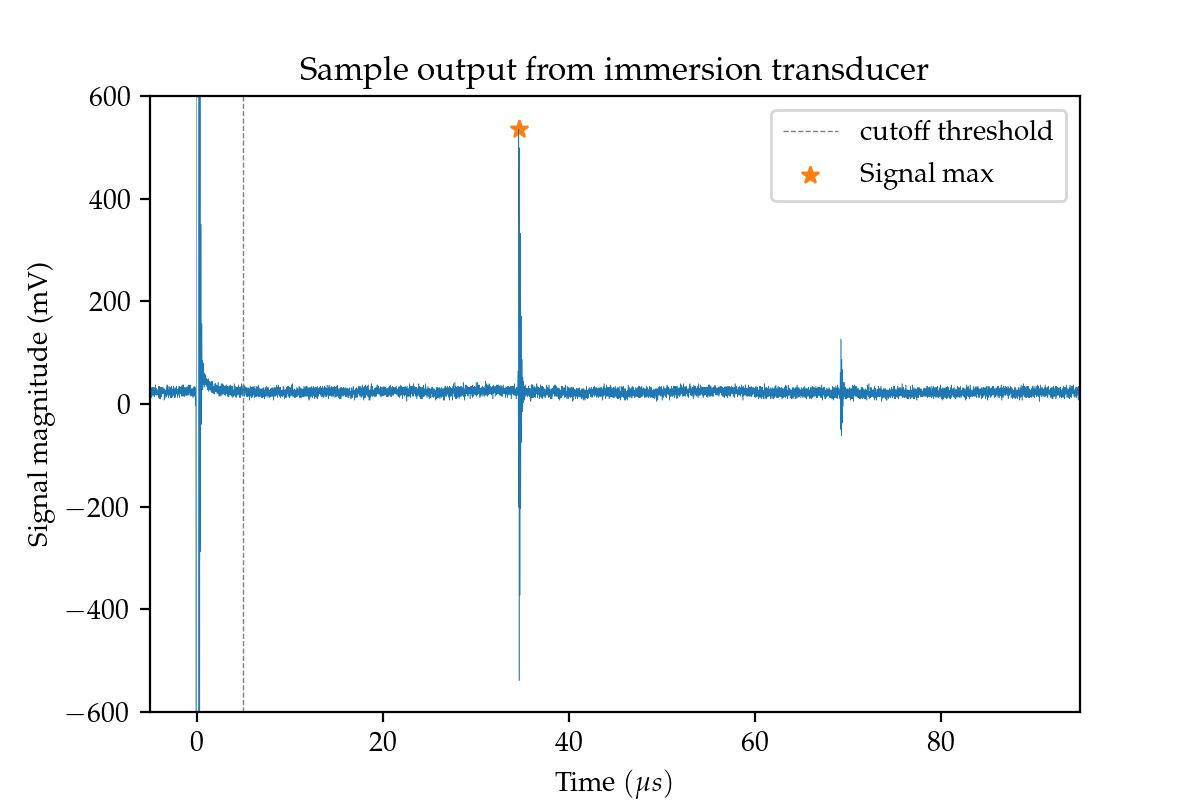
\includegraphics[width=.75\linewidth]{figures/IT_sample_1.jpg}
    \caption{Sample output from the immersion transducer, and the output of a naive fitness function.}\label{fig:immersionTransducerSample}
\end{center}
\end{figure}

As mentioned previously the data in \autoref{fig:fullscan-6} spans a search space of $28 mm$ in the translational $z$ axis and $26^\circ$ in the rotational $\theta_x$ and $\theta_y$ axes. The translational $x$ and $y$ axes were omitted because the bottom of the tank the transducer was bouncing off of was flat, so motion in this plane would have no bearing on the output signal strength.
We focus the transducer ahead of starting the scan so that we could minimize the size of the search area we needed to look through while still capturing the full shape of the fitness function as it falls off from a fully-focused position to a position where the noise completely blots out the signal.

Higher-resolution data provides us more information about the shape of the fitness function as well as its sensitivity to noise, but the number of points the fullscan needs to visit grows exponentially as the resolution shrinks.
The \texttt{test\_6.json} data has a resolution of $1.0^\circ$ in the rotational axes and $0.4 mm$ in the translational axis; since there are two translational and one rotational axis, the total number of points was equal to $\left(\frac{26}{1} + 1\right) \cdot \left(\frac{26}{1} + 1\right) \cdot \left(\frac{28}{0.4} + 1\right) = 51,759$ (Plus-one is added to each range since the motion of the robot includes endpoints)

Since the cost of increased resolution is so high, the resolution and search space volume should be calibrated to capture the minimum number of points that provide you all the information you need about the fitness function. If you know the signal you're measuring falls off within $1.1mm$ of the focal point, don't expand the search space any further than that.

\subsubsection{Parsing a high-resolution scan}
The full-scan module captures a very large amount of data, but most of it is

\begin{center}
    \begin{tikzpicture}[
        node distance=1cm,
        % >={Triangle[angle=60:1pt 2]},
        shorten >= 2pt,
        shorten <= 2pt,
        arrow/.style={
        ->,
        line width=2pt
        }]
        
        \node[block] (A) {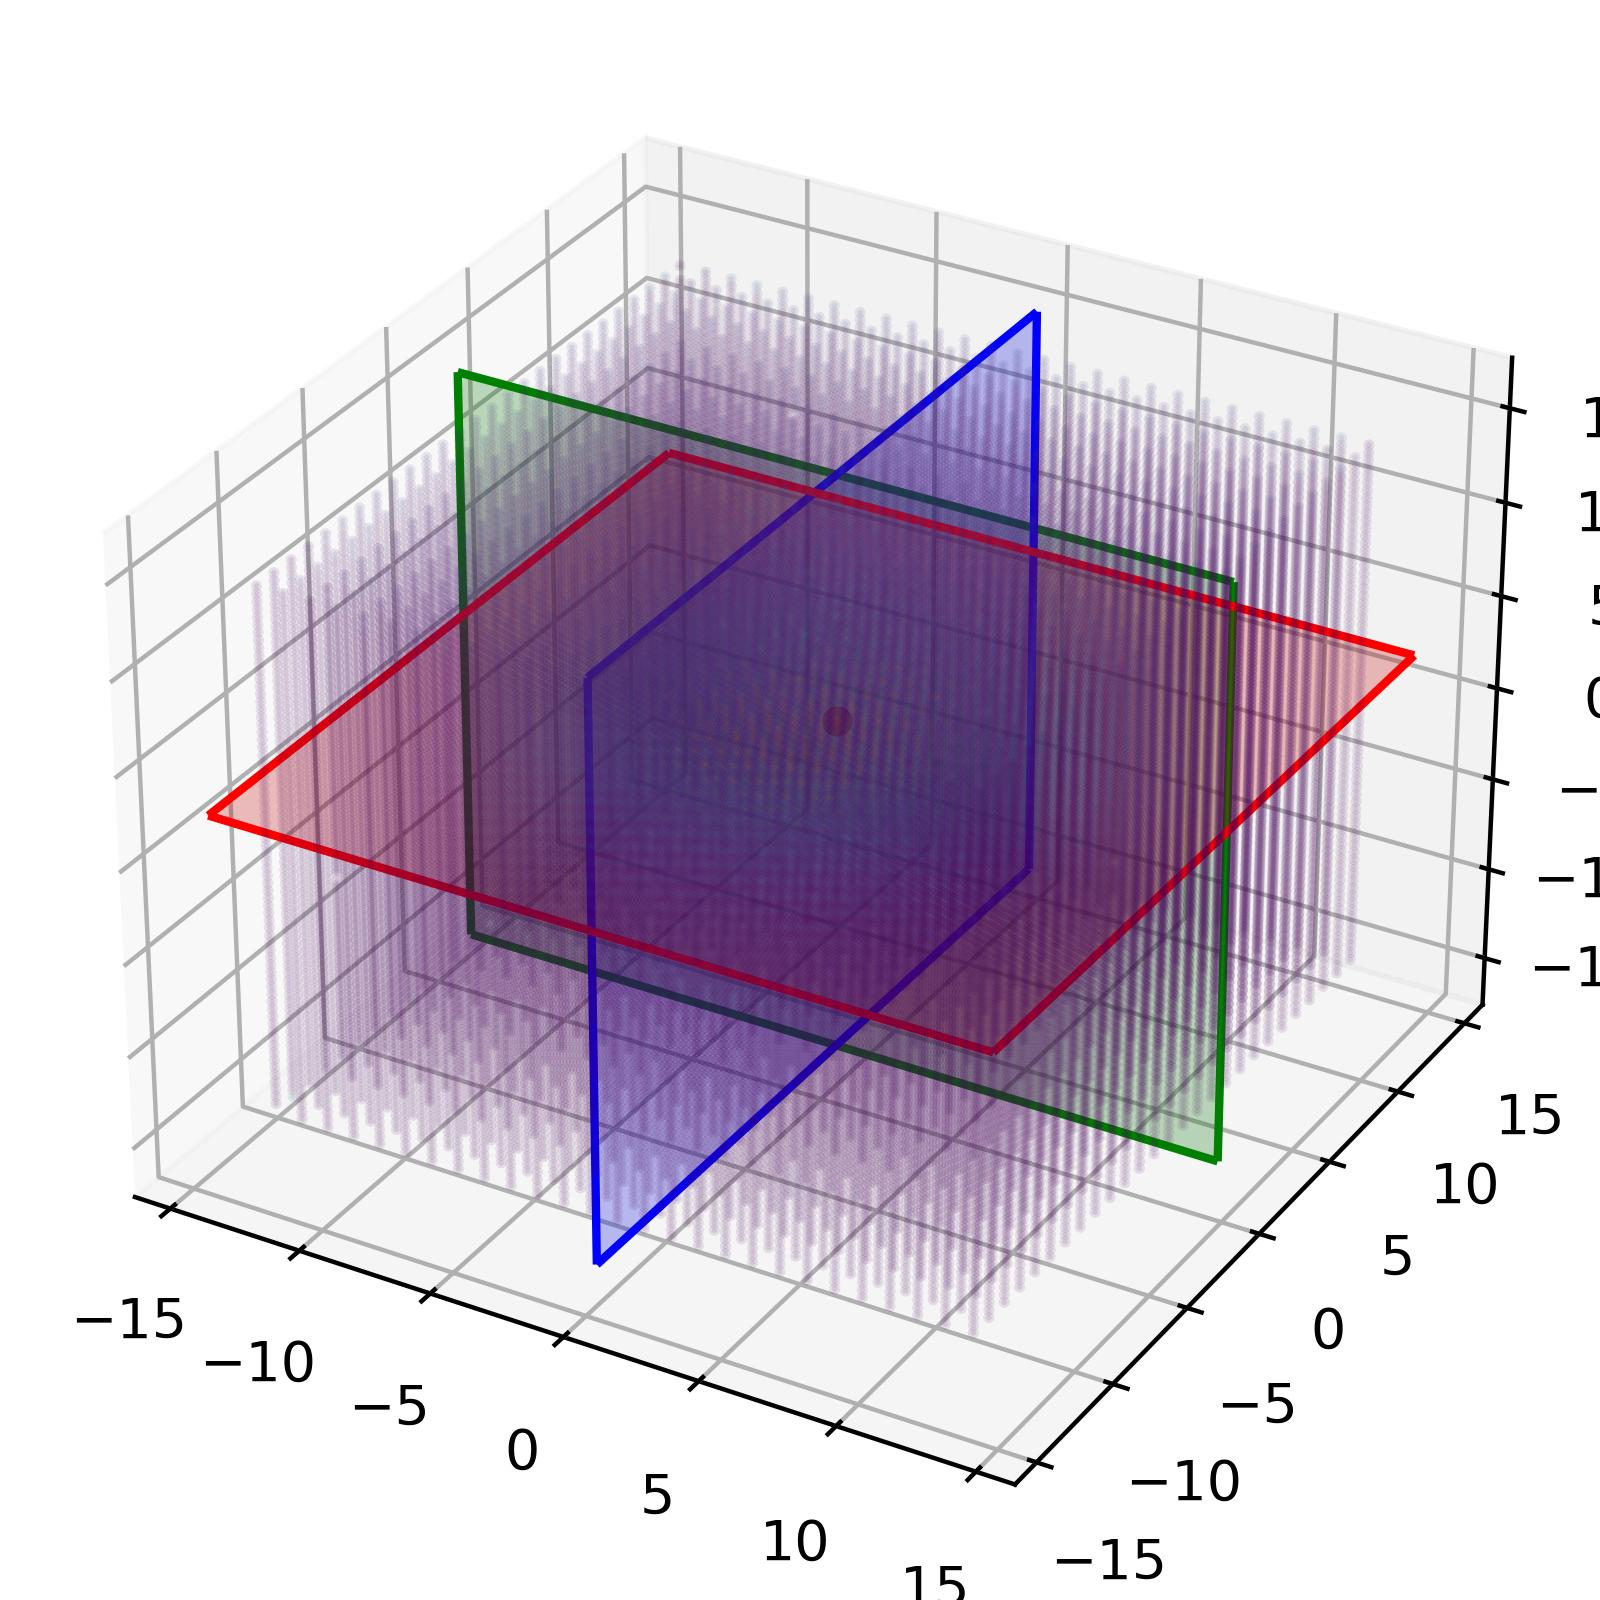
\includegraphics[width=4cm,height=4cm]{figures/data_slice1_6.jpg}};
        \node[block,below=of A] (B) {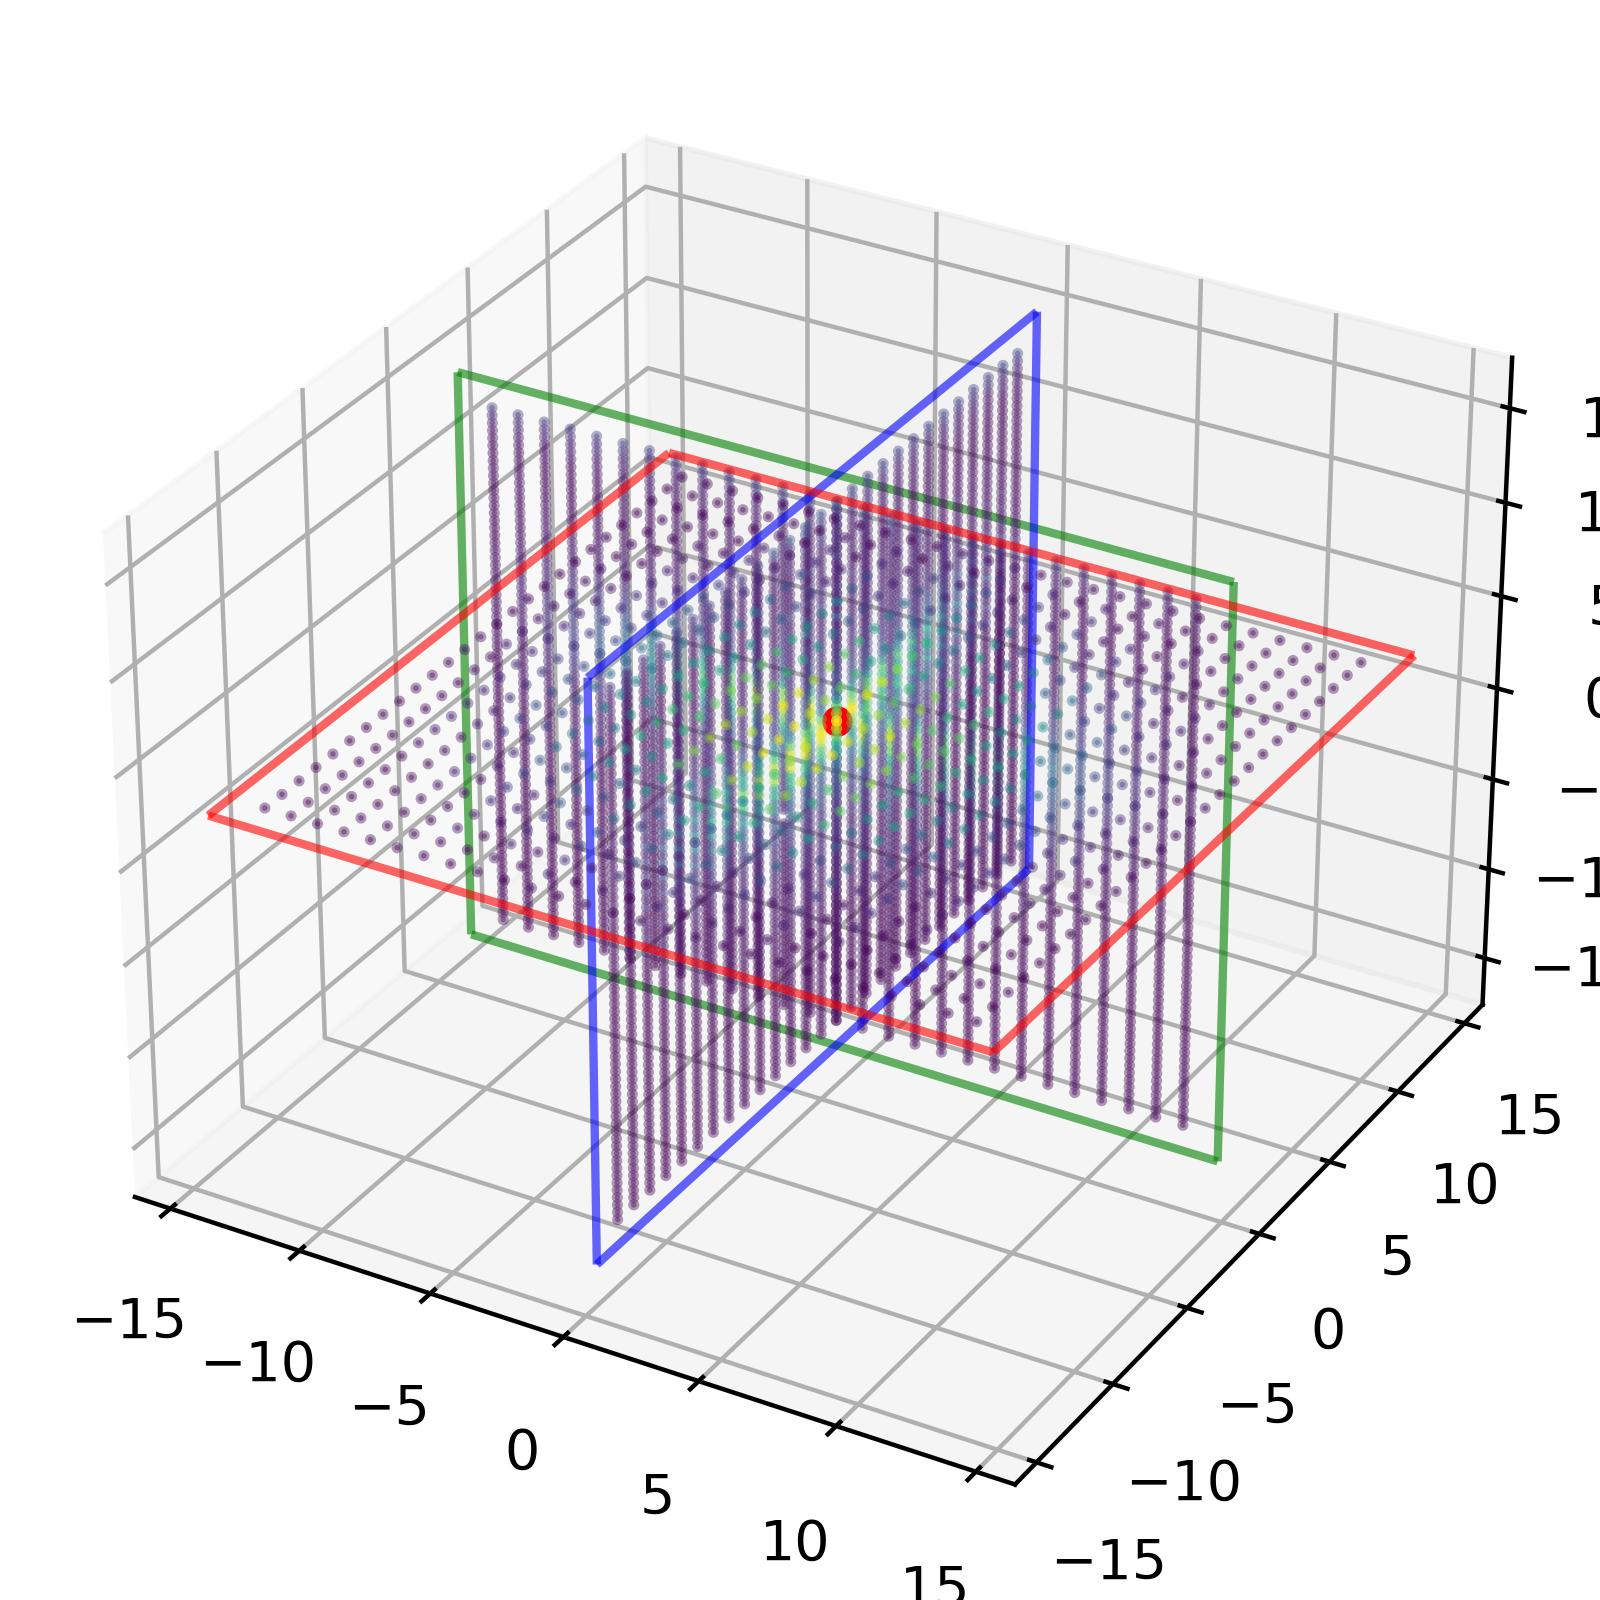
\includegraphics[width=4cm,height=4cm]{figures/data_slice2_6.jpg}};
        \node[block,below=of B] (D) {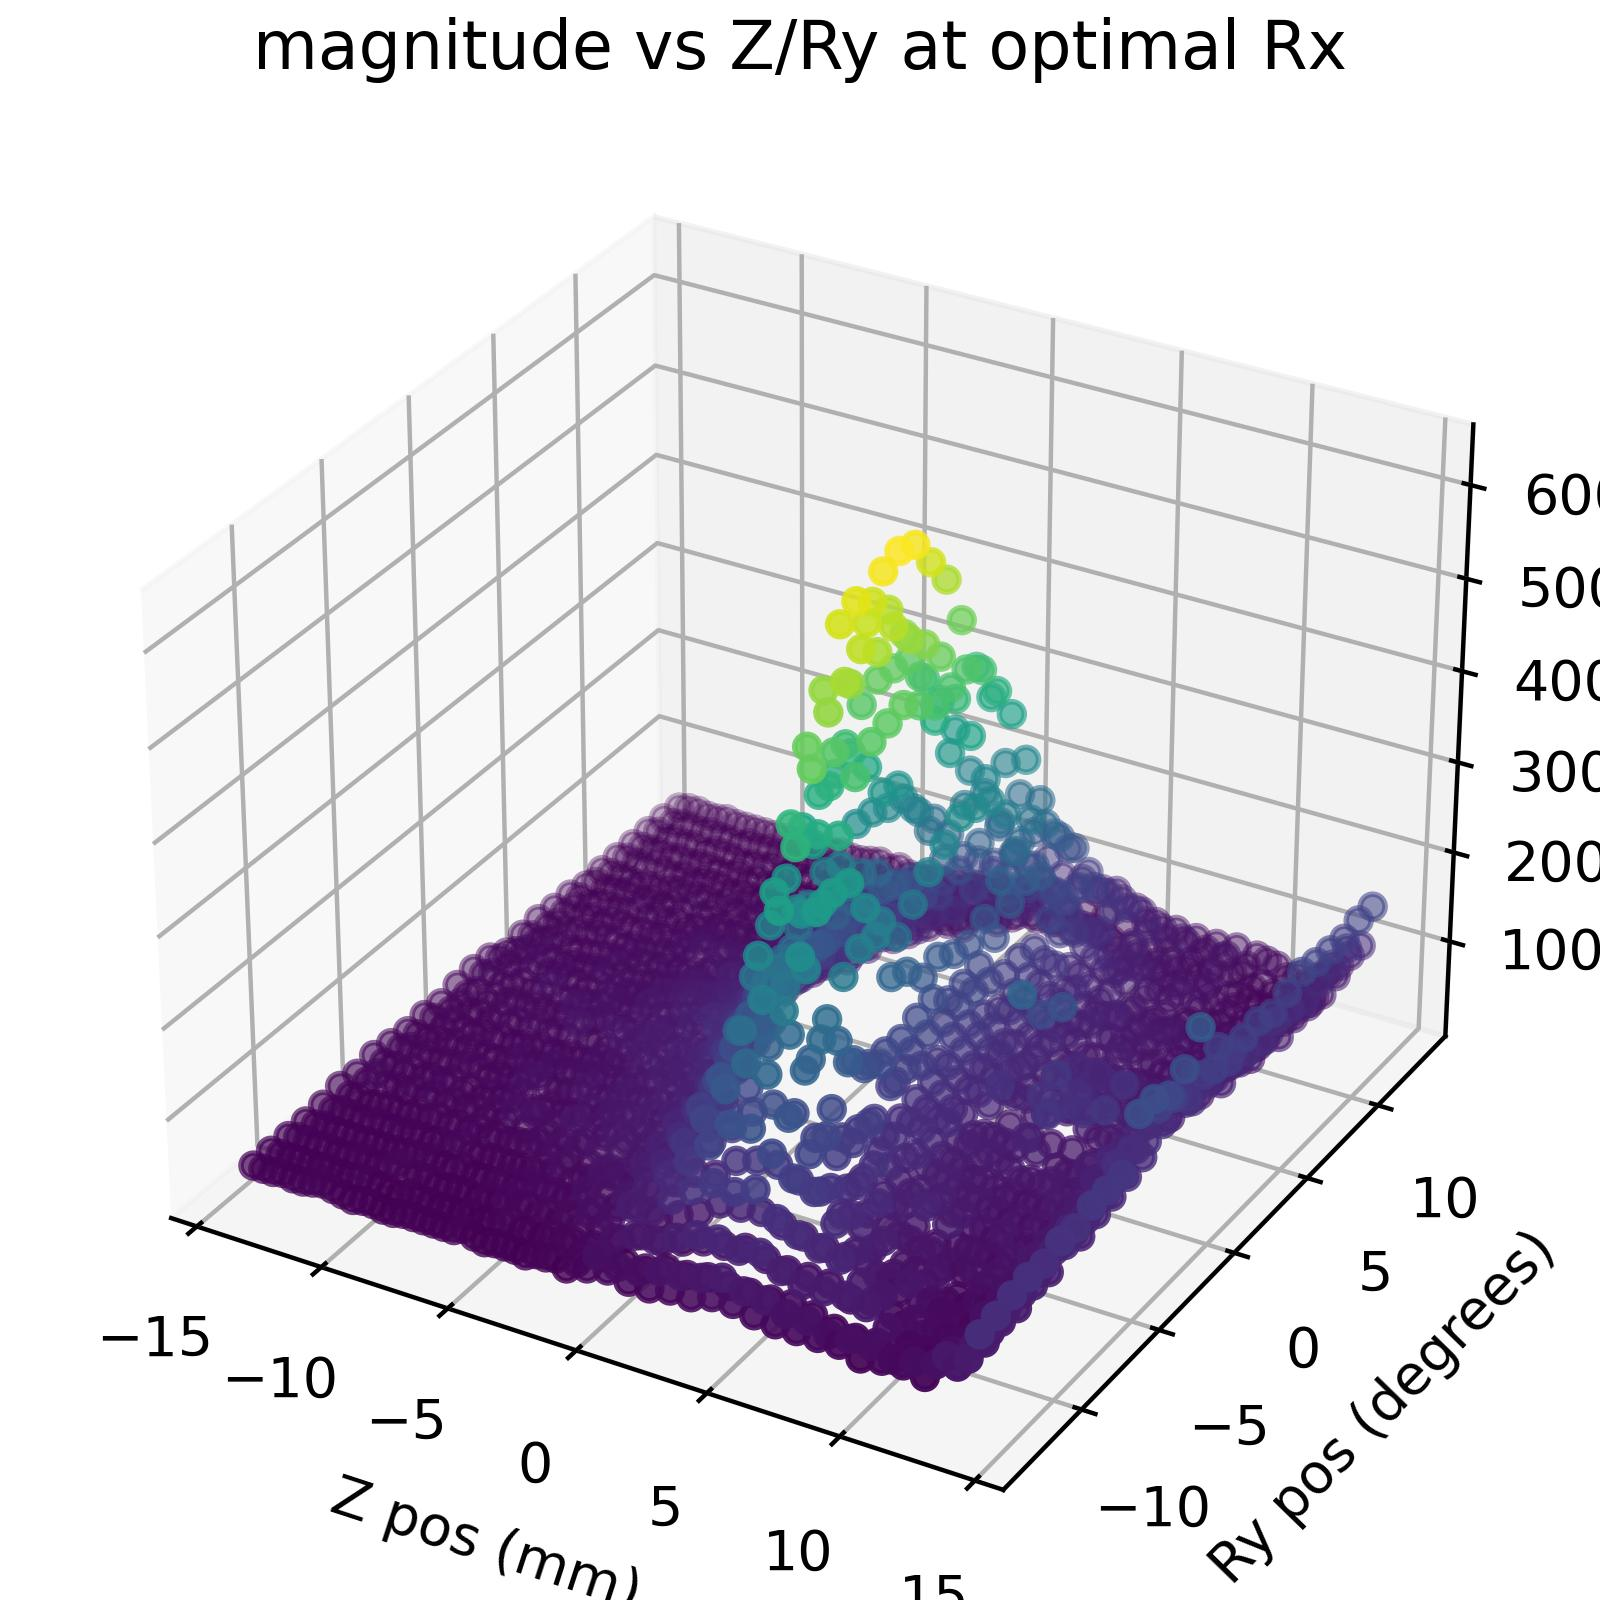
\includegraphics[width=4cm,height=4cm]{figures/Isolated_axes_2_6.jpg}};
        \node[block,left=of D] (C) {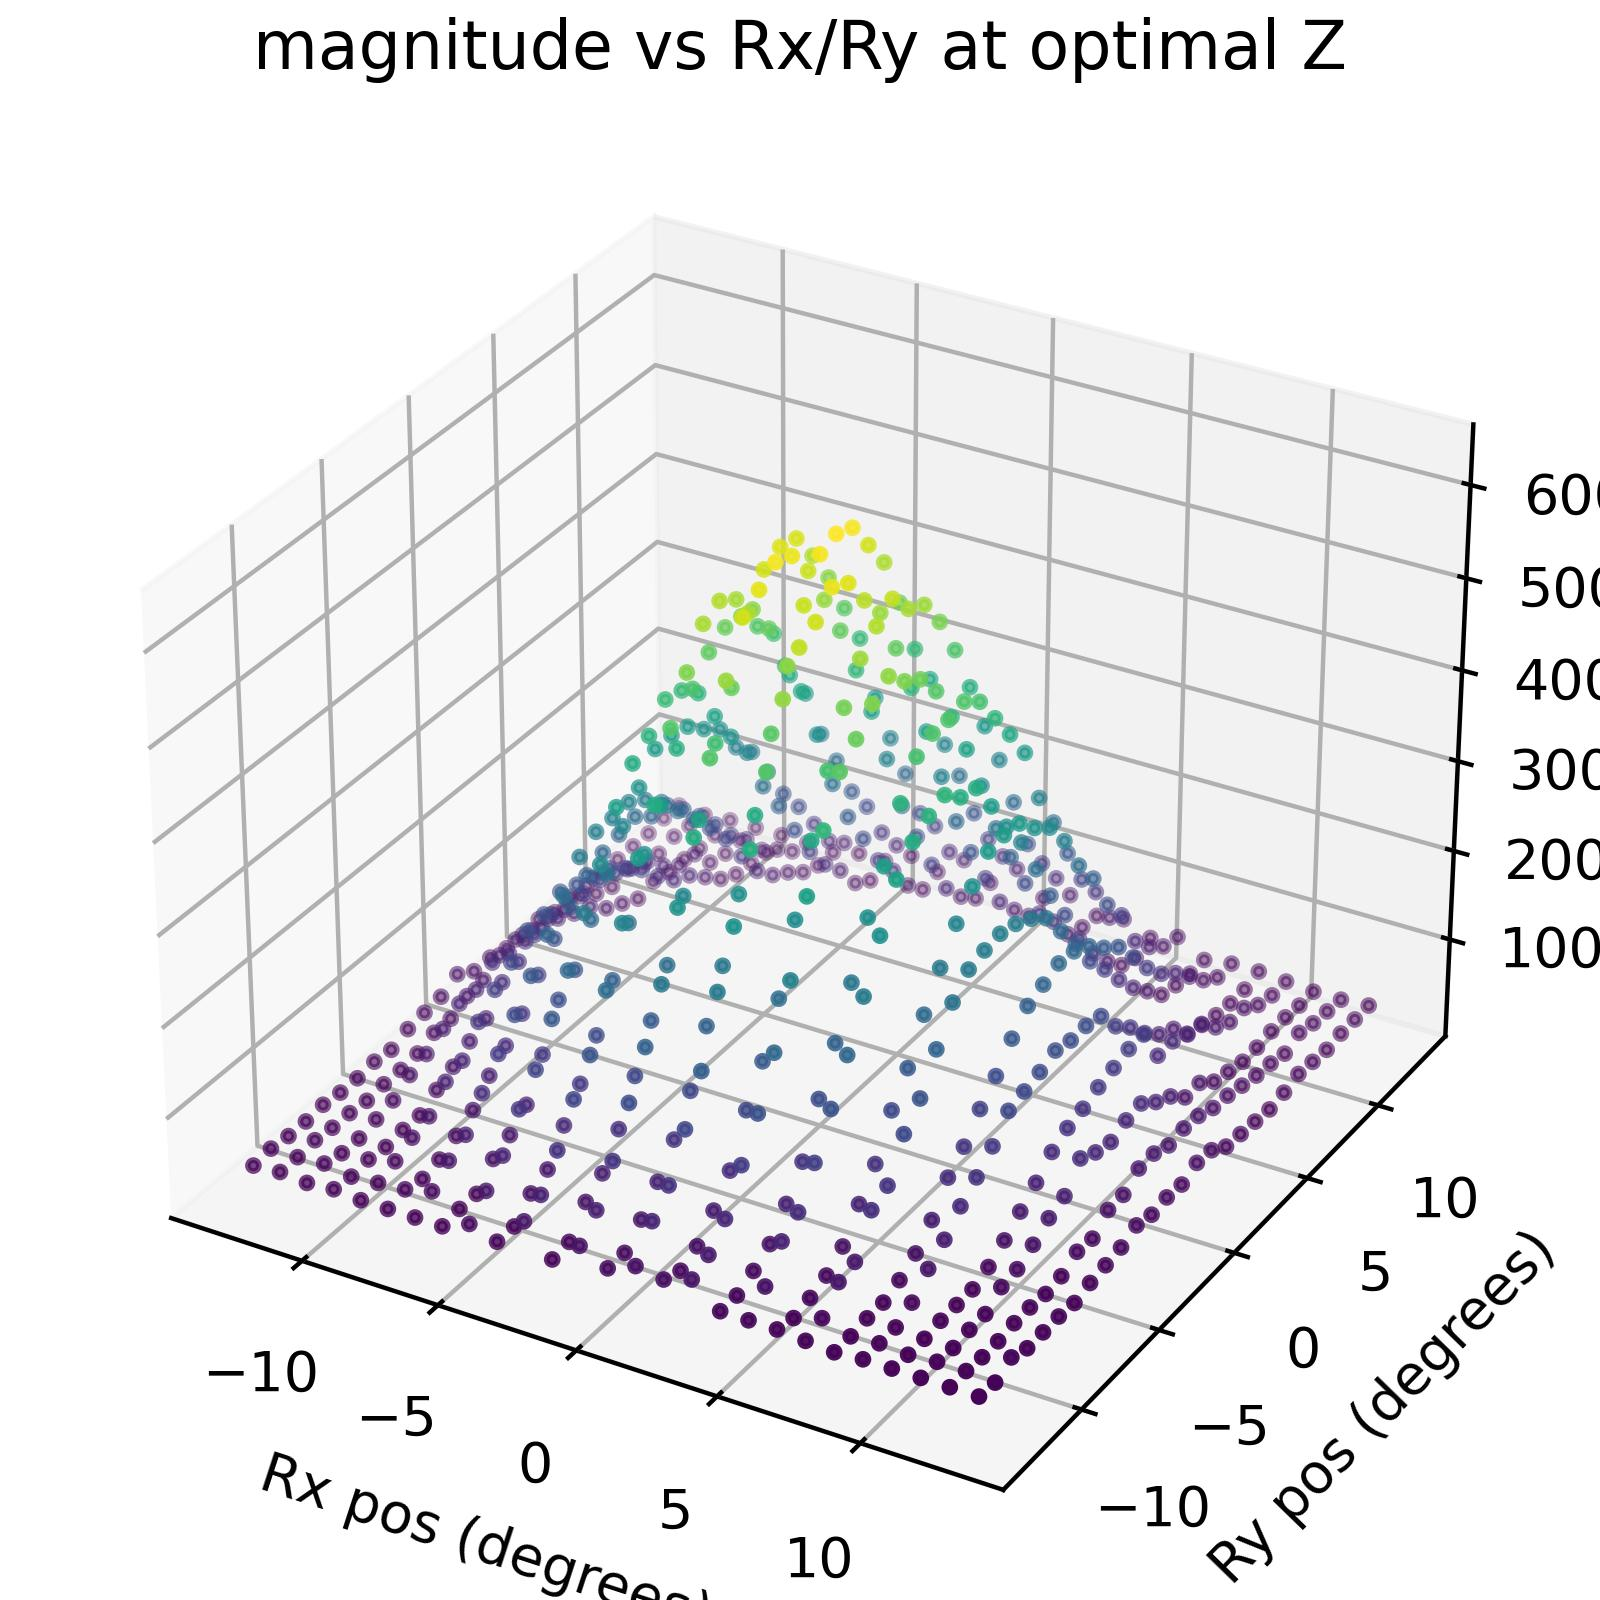
\includegraphics[width=4cm,height=4cm]{figures/Isolated_axes_1_6.jpg}};
        \node[block,right=of D] (E) {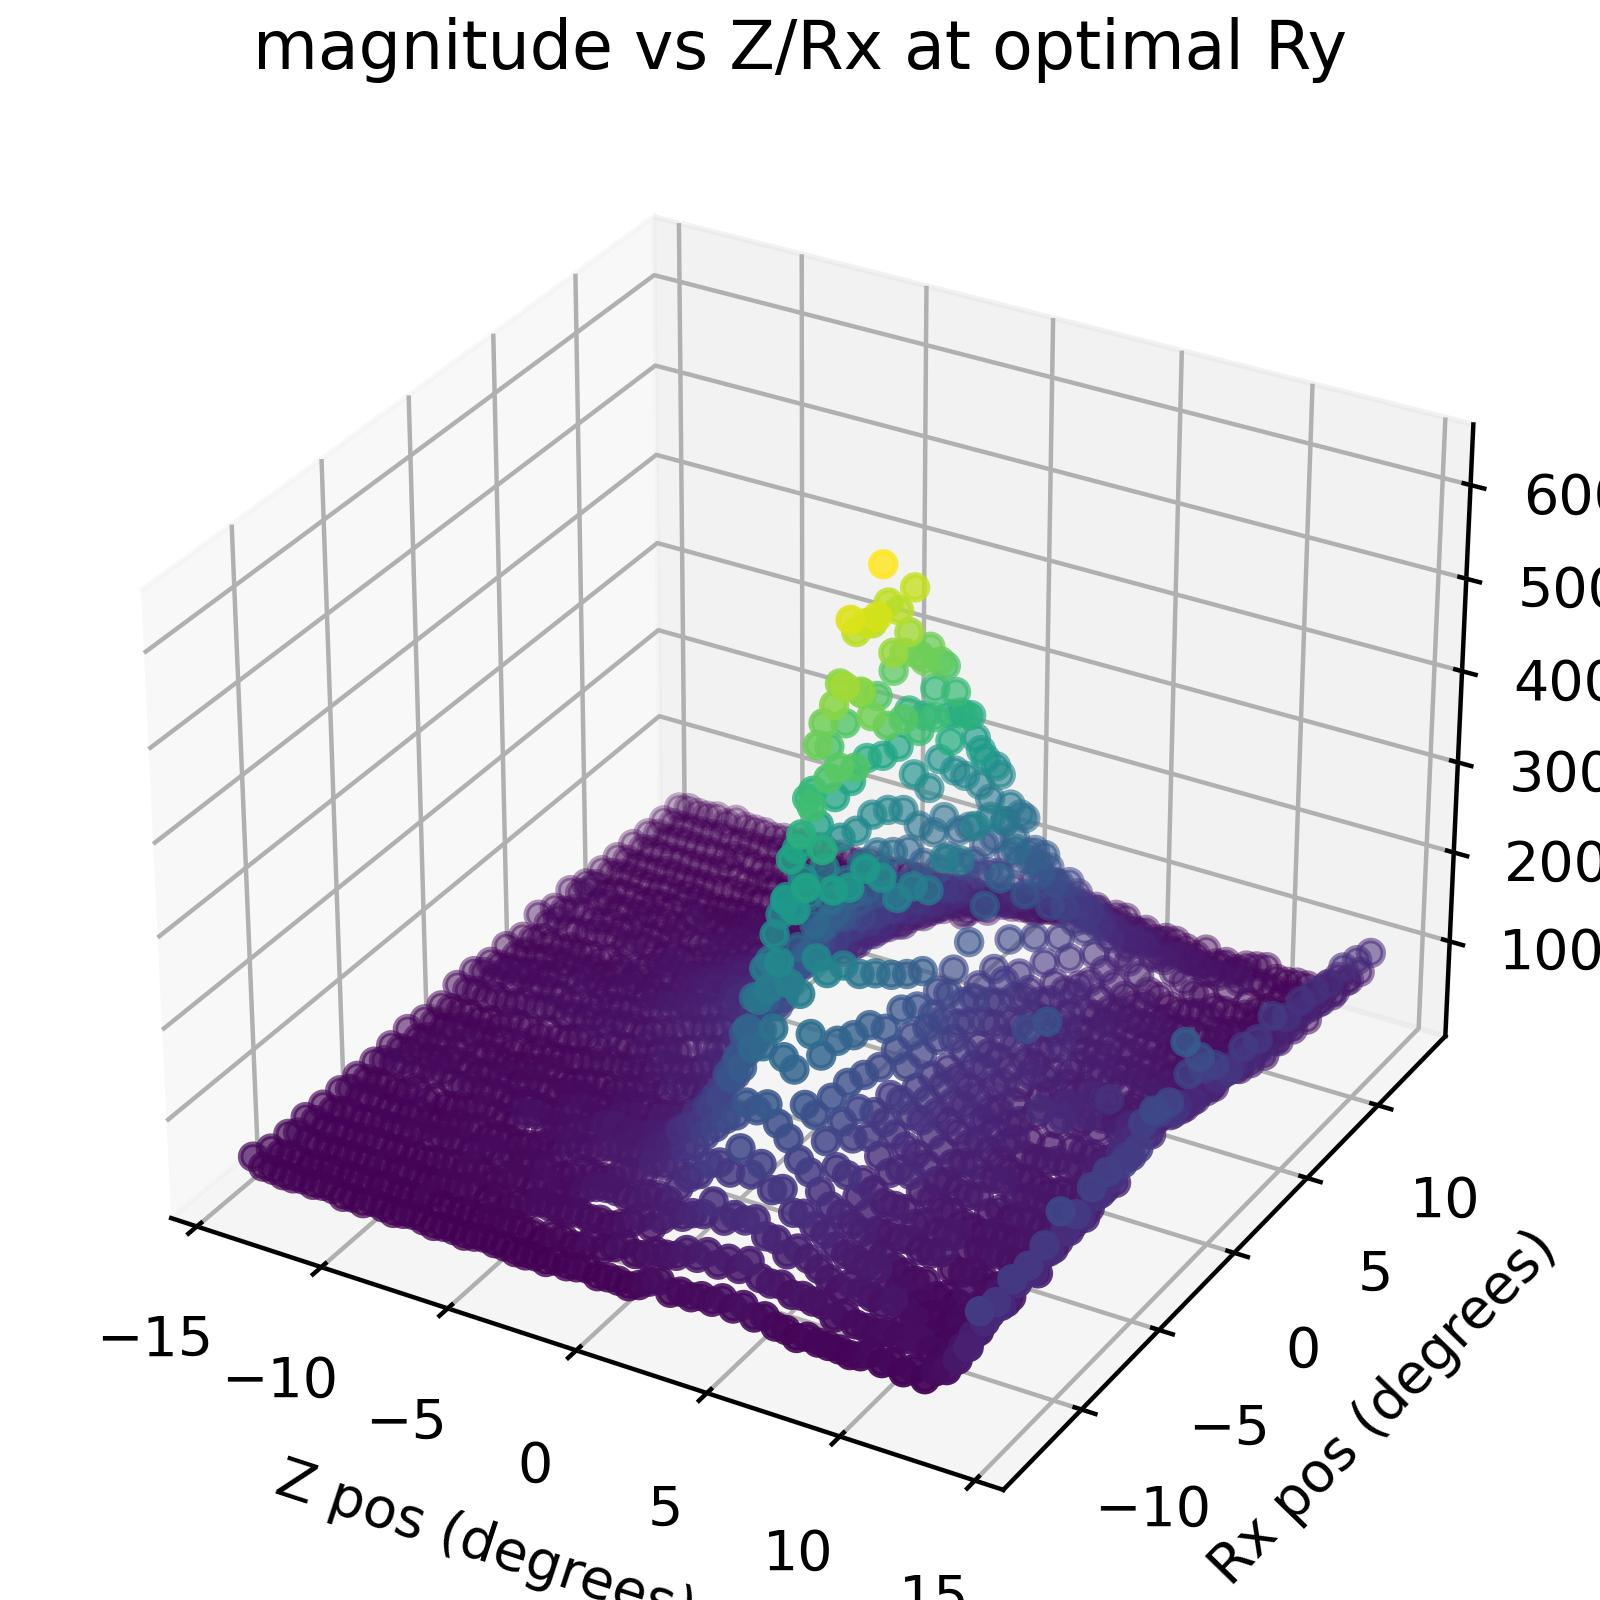
\includegraphics[width=4cm,height=4cm]{figures/Isolated_axes_3_6.jpg}};

        \draw[arrow]
        (A) -- (B);
        \draw[red, arrow]
        (B) -- (C);
        \draw[blue, arrow]
        (B) -- (D);
        \draw[green, arrow]
        (B) -- (E);

    \end{tikzpicture}
\end{center}

\end{document}